\documentclass[tikz]{standalone}
\usetikzlibrary{patterns}
\usetikzlibrary{arrows}
\usetikzlibrary{decorations.shapes,decorations.markings,decorations.pathreplacing}

\tikzset{
    set arrow inside/.code={\pgfqkeys{/tikz/arrow inside}{#1}},
    set arrow inside={end/.initial=>, opt/.initial=},
    /pgf/decoration/Mark/.style={
        mark/.expanded=at position #1 with
        {
            \noexpand\arrow[\pgfkeysvalueof{/tikz/arrow inside/opt}]{\pgfkeysvalueof{/tikz/arrow inside/end}}
        }
    },
    arrow inside/.style 2 args={
        set arrow inside={#1},
        postaction={
            decorate,decoration={
                markings,Mark/.list={#2}
            }
        }
    },
}
\begin{document}

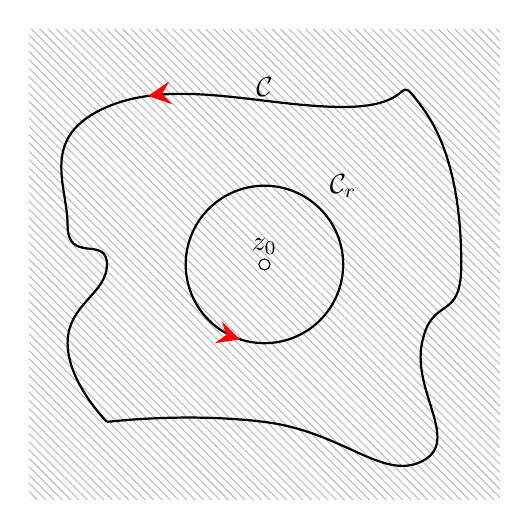
\begin{tikzpicture}
\draw[pattern=north west lines,pattern color=gray!50,draw=white] (-3,-3) -- (-3,3) -- (3,3) -- (3,-3) -- (-3,-3);
%\draw[->,thick,gray] (-2,0) -- (1.75,0) node[right]{$\mathrm{Re}$};
%\draw[->,thick,gray] (0,-2) -- (0,1.75) node[above]{$\mathrm{Im}$};
\draw[fill=white] (0,0) circle (2pt) node[above] {$z_0$};
\draw[thick] plot [smooth,tension=0.9] coordinates {(-2,-2) (0,-2) (2,-2.5) (2,-1) (2.5,0) (2,2) (1,2) (-2,2) (-2.5,0.5) (-2,0) (-2.5,-1) (-2,-2)} [arrow inside={end=stealth,opt={red,scale=2}}{0.7}];
\draw[thick] (0,0) circle (1) [arrow inside={end=stealth,opt={red,scale=2}}{0.7}];
\draw (1,1) node{$\mathcal{C}_r$};
\draw (0,2.25) node {$\mathcal{C}$};
%\draw (-2,-2) node[below]{$\mathcal{C}$};
%\draw[thick,dashed,fill=white] (0,0) circle (2);
%\draw[fill] (0,0) circle (2pt);
%\draw[fill] (-4.5,2) circle (2pt);
%\draw (-4.5,2) -- (0,0);
\end{tikzpicture}

\end{document}